\documentclass[11pt]{scrartcl}
\usepackage[utf8]{inputenc}
\usepackage[T1]{fontenc}
\usepackage{dirtree}
\usepackage[ngerman]{babel}
\usepackage{listings, color}
\usepackage{graphicx}

\graphicspath{ {./images/} }


\lstdefinestyle{test}
{
    basicstyle=\ttfamily
}
\lstdefinestyle{Bash}
{
    language=bash,
    frame=lrtb,
    basicstyle=\ttfamily,
    showstringspaces=false,
    keywordstyle=\color{blue}
}
\lstdefinestyle{gdisk}
{
    basicstyle=\ttfamily,
    showstringspaces=false,
    commentstyle=\color{red},
    keywordstyle=\color{blue}
}

\author{Sebastian Knauer}
\title{Installation und Konfiguration von Arch Linux}
\begin{document}
\maketitle

\includegraphics[scale=0.75]{arch-logo.pdf}

\section{Einleitung}
\label{sec:einleitung}
Anleitung für Arch-Setup mit folgender Hardware:
\begin{itemize}
    \item Acer Aspire 5942G-724G32MN
    \item Samsung SSD 840 Evo 120GB 
    \item BenQ Full HD Monitor 
    \item Canon Pixma MG5350 Drucker
\end{itemize}


\section{Basissystem}
\label{sec:base-system}
Nach dem Bootvorgang ist man als root eingeloggt.
Lade deutsches Tastaturlayout:
\begin{lstlisting}[style=Bash]
# loadkeys de
# loadkeys de-latin1
\end{lstlisting}

\subsection{Netzwerk}
\label{subsec:network}
Ist Ethernet Netzwerkkarte geladen?
\begin{lstlisting}[style=Bash]
# ip link 
\end{lstlisting}
Wenn nein, Modul herausfinden:
\begin{lstlisting}[style=Bash]
# lspci -v | less 
\end{lstlisting}
Fehlermeldung des Moduls analysieren:
\begin{lstlisting}[style=Bash]
# dmesg | grep tg3 
\end{lstlisting}
Modul erneut laden
\begin{lstlisting}[style=Bash]
# modprobe -r tg3
# modprobe tg3
\end{lstlisting}
Verfizieren:
\begin{lstlisting}[style=Bash]
# dmesg | grep tg3 
# ip link
\end{lstlisting}

\subsection{Partitionierung}
\label{subsec:partitioning}
Die Partitionstabelle wird mit dem GPT erstellt.
Nur root partition und swap(1gb) sowie boot partition(3MB), 
da wenig speicherplatz.

\begin{lstlisting}[style=Bash]
# gdisk /dev/sda
\end{lstlisting}
\begin{lstlisting}[style=gdisk]
o           :alles loeschen
p           :Partitionsschema anzeigen

n           :neue Partition (root-Partition)
<default>   :Sollte 1 sein
<default>     
+110G       :Partition auf 110 GB setzen
<default>   :8300 (linux file system)

n           :neue Partition (swap-Partition)
<default>   :Sollte 3 sein
<default>     
+1G         :Partition auf 3 GB setzen
8200        :swap

n           :neue Partition (boot-Partition)
128         
-3M         :Partition auf 3MB setzen
<default>   
ef02        :Gpt boot

w           :schreiben und speichern
\end{lstlisting}
Filesysteme erstellen:
\begin{lstlisting}[style=Bash]
# mkfs.ext4 -L arch /dev/sda1
# mkswap -L swap /dev/sda2
# swapon /dev/sda2
\end{lstlisting}
Partitionen mounten:
\begin{lstlisting}[style=Bash]
# mount /dev/sda1 /mnt 
\end{lstlisting}

\subsection{Installation}
\label{subsec:installation}
\begin{lstlisting}[style=Bash]
# pacstrap /mnt base base-devel 
# genfstab -Up /mnt > /mnt/etc/fstab 
\end{lstlisting}

\subsection{Koniguration}
\label{subsec:config}
\begin{lstlisting}[style=Bash]
# arch-chroot /mnt/ /bin/bash
\end{lstlisting}
\begin{lstlisting}[style=Bash]
# echo $hostname$ > /etc/hostname
# echo LANG=de_DE.UTF-8 > /etc/locale.conf
# echo KEYMAP=de-latin1 > /etc/vconsole.conf
# ln -s /usr/share/zoneinfo/Europe/Berlin /etc/localtime
\end{lstlisting}
Bearbeite /etc/locale.gen
\begin{lstlisting}[style=Bash]
/etc/locale.gen
!\dotfill!
de_DE.UTF-8 UTF-8
de_DE ISO-8859-1
de_DE@euro ISO-8859-15
\end{lstlisting}
\begin{lstlisting}[style=Bash]
# locale-gen 
\end{lstlisting}
Uncomment multilib in /etc/pacman.conf
\begin{lstlisting}[style=Bash]
...
[multilib]
Include = /etc/pacman.d/mirrorlist
...
\end{lstlisting}
Kernel erstellen
\begin{lstlisting}[style=Bash]
# mkinitcpio -p linux
\end{lstlisting}
Root password setzen 
\begin{lstlisting}[style=Bash]
# passwd
\end{lstlisting}
Bootloader installieren und konfigurieren
\begin{lstlisting}[style=Bash]
# pacman -S grub 
# grub-install /dev/sda 
\end{lstlisting}
DPM Dekativieren in /etc/default/grub, da es sehr langsam ist:
\begin{lstlisting}[style=Bash]
...
GRUB_CMDLINE_LINUX_DEFAULT="quiet radeon.dpm=0"
...
# grub-mkconfig -o /boot/grub/grub.cfg 
\end{lstlisting}
Finish it:
\begin{lstlisting}[style=Bash]
# exit 
# umount -R /mnt
# reboot 
\end{lstlisting}

\section{Post-Install Konfiguration}
\begin{lstlisting}[style=Bash]
# systemctl enable dhcpcd
\end{lstlisting}
\begin{lstlisting}[style=Bash]
# useradd -m -g users -s /bin/bash sebastian 
# passwd sebastian
# usermod -aG wheel sebastian
\end{lstlisting}
Uncomment wheel group in /etc/sudoers with nopasswd:
\begin{lstlisting}[style=Bash]
# visudo 
...
%wheel ALL=(ALL) NOPASSWD: ALL
...

\end{lstlisting}
Uhrzeit:
\begin{lstlisting}[style=Bash]
# pacman -S ntp 
# vi /etc/ntp.conf

server time.zih.tu-dresden.de
server de.pool.ntp.org

# systemctl enable ntpd 
\end{lstlisting}
Pacman Wundstrasse, TuDresden Mirror in /etc/pacman.d/mirrorlist
\begin{lstlisting}[style=Bash]

...
server = ftp://ftp.wh2.tu-dresden.de/pub/mirrors
/archlinux/$repo/os/x86_64
...

$
\end{lstlisting}
Sound:
\begin{lstlisting}[style=Bash]
# pacman -S alsa-utils 
$ alsamixer
$
\end{lstlisting}
'm' drücken um Master Channel zu unmuten

\subsection{X11}
\label{sec:x11}
Installiere Xorg-server, Graphikkartentreiber, Windowmanager und Touchpadtreiber:
\begin{lstlisting}[style=Bash]
# pacman -S xorg-server xorg-server-utils xorg-xinit 
# pacman -S mesa xf86-video-ati lib32-ati-dri
# pacman -S i3
# pacman -S xf86-input-synaptics
\end{lstlisting}
Füge ans Ende der \emph{.xinitrc} i3 als wm ein:
\begin{lstlisting}[style=Bash]
$ vi .xinitrc 

...
xrandr --output LVDS --off --output HDMI-0 --auto
exec i3
$
\end{lstlisting}
Wallpaper: 
\begin{lstlisting}[style=Bash]
# pacman -S feh
# systemctl enable cronie
$ crontab -e
...
*/15 * * * * DISPLAY=:0.0 feh --bg-scale /home/sebastian/Bilder/Wallpaper
...
$
\end{lstlisting}
Der X-Server wird gestartet
\begin{lstlisting}[style=Bash]
$ startx
...
$
\end{lstlisting}

    
\section{Programme und Konfiguration}
\label{sec:programme}
\graphicspath{ {programme/images/} }

\subsection{Texteditor}
\begin{tabular}{l|l}
Paketname & \textbf{vim} \\ 
Konfigurationsdatei & {{\raise.17ex\hbox{$\scriptstyle\mathtt{\sim}$}}/.vimrc} \\
\end{tabular}
\\ \\
Verzeichnisstruktur:  
\dirtree{%
    .1 /.
    .2 .vim.
    .3 colors.
    .3 ftplugin.
}

\subsection{Terminal Emulator}
\begin{tabular}{l|l}

\includegraphics[scale=0.75]{urxvt-logo.pdf} & Urxvt \\ \hline
Paketname & \textbf{rxvt-unicode} \\ 
Repository & official repository(community) \\
Konfigurationsdatei & {{\raise.17ex\hbox{$\scriptstyle\mathtt{\sim}$}}/.Xdefaults} \\
Lizenz & GPL \\
Besonderheiten & schnell \\
\end{tabular}
\\ \\
Er wird also Daemon gestartet: 
\begin{lstlisting}[style=Bash]
# systemctl start urxvtd@username.service
# systemctl enable  urxvtd@username.service
\end{lstlisting}
In der \emph{.bashrc} muss er, der client, nun als Umgebungsvarible definiert werden:
\begin{lstlisting}[style=Bash]
$ vim .bashrc 

...
export TERMINAL=urxvtc
...

$
\end{lstlisting}

\subsection{Windowmanager}
\begin{tabular}{l|l}

\includegraphics[scale=0.2]{i3-logo.png} & i3 - improved tiling wm \\ \hline
Paketname & \textbf{i3} (Paketgruppe) \\ 
Repository & official repository(community) \\
Konfigurationsdatei & {{\raise.17ex\hbox{$\scriptstyle\mathtt{\sim}$}}/.i3/config} \\
Lizenz & BSD \\
Besonderheiten & schnell \\
\end{tabular}
\\ \\
Erste shortcuts definieren:

\begin{lstlisting}[style=Bash]
$ vim .i3/conifg

...
bindsym XF86AudioRaiseVolume exec amixer -q sset Master 1+ unmute
bindsym XF86AudioLowerVolume exec amixer -q sset Master 1- unmute
bindsym XF86AudioMute exec amixer -q sset Master toggle
...

$
\end{lstlisting}

\subsection{Filemanager}
\begin{tabular}{l|l|l}
Paketname & \textbf{pcmanfm} & \textbf{vifm} \\ 
Konfigurationsdatei & {{\raise.17ex\hbox{$\scriptstyle\mathtt{\sim}$}}.config/pcmanfm/default/pcmanfm.conf} &
{{\raise.17ex\hbox{$\scriptstyle\mathtt{\sim}$}}/.vifm/vifmrc} \\
\end{tabular}
\\ \\
Opening filetypes eintragen:
\begin{lstlisting}[style=Bash]
$ vim .vifm/vifmrc

...
filetype *.pdf evince %f

$
\end{lstlisting}
Für networking-Unterstützung müssen zusätzliche Pakete installiert werden:
\begin{lstlisting}[style=Bash]
# pacman -S gvfs gvfs-smb 
\end{lstlisting}

\subsection{Webbrowser}
\begin{tabular}{l|l|l}

\includegraphics[scale=0.1]{chromium-logo.pdf} & Chromium & Flash-Support \\ \hline
    Paketname & \textbf{chromium} & \textbf{chromium-pepper-flash} \footnote{pacaur erst installieren} \\ 
Repository & official repository(extra) & arch user repository \\
Konfigurationsdatei & - & - \\
Lizenz & BSD & custom: chrome  \\
Besonderheiten & schnell, addons:adblock, youtube unblocker \\
\end{tabular}

\subsection{AUR-Helper}
Pacaur \textbf{pacaur} muss aus dem AUR heruntergeladen und selbst gebuildet werden.
Zunächst jedoch muss \textbf{expac} aus den official repositories installiert werden.
\begin{lstlisting}[style=Bash]
# pacman -S expac
\end{lstlisting}
Danach muss \textbf{cower} aus dem AUR heruntergeladen und installiert werden:
\begin{lstlisting}[style=Bash]
$ wget https://aur.archlinux.org/packages/co/cower/cower.tar.gz
$ tar -xf cower.tar.gz
$ cd cower
$ makepkg
# pacman -U cower-$version-$arch.pkg.tar.xz
\end{lstlisting}
Schließlich muss pacaur selbst aus dem AUR heruntergeladen und installiert werden:
\begin{lstlisting}[style=Bash]
$ wget https://aur.archlinux.org/packages/pa/pacaur/pacaur.tar.gz
$ tar -xf pacaur.tar.gz
$ cd pacaur
$ makepkg
# pacman -U pacaur-$version-$arch.pkg.tar.xz
\end{lstlisting}

\subsection{\LaTeX}
\begin{tabular}{l|l}

\includegraphics[scale=0.05]{latex-logo.pdf} & \LaTeX \\ \hline
Paketname & \textbf{texlive-core} \\ 
Repository & official repository(extra) \\
Konfigurationsdatei & - \\
Lizenz & GPL \\
Besonderheiten & - \\
\end{tabular}
\\ \\
\emph{.sty}-files kommen nach \emph{texmf/tex/latex/local}.
Mit 
\begin{lstlisting}[style=Bash, frame=none]
$ texhash
$
\end{lstlisting}
wird die Latex database aktualisiert.
\dirtree{%
    .1 /.
    .2 texmf.
    .3 tex.
    .4 latex.
    .5 local.
}

\subsection{PDF-Viewer}
\begin{tabular}{l|l}

\includegraphics[scale=1]{evince-logo.pdf} & Evince \\ \hline
Paketname & \textbf{evince} \\ 
Repository & official repository(extra) \\
Konfigurationsdatei & - \\
Lizenz & GPL \\
Anmerkung & Gute balance zwischen performance und funcionality \\
\end{tabular}

\subsection{Backup-tool}
\begin{tabular}{l|l}
Paketname & \textbf{rsnapshot} \\ 
Konfigurationsdatei & /etc/rsnapshot.conf \\
\end{tabular}
Es kann eine Datei *.exclude angelegt werden. Der pfad wird in der Konfigurationsdatei spezifiziert

\subsection{E-mail client}
\begin{tabular}{l|l}

\includegraphics[scale=0.75]{thunderbird-logo.pdf} & Thunderbird \\ \hline
Paketname & \textbf{thunderbird} \\ 
Repository & official repository(extra) \\
Konfigurationsdatei & - \\
Lizenz & GPL,MPL \\
Besonderheiten & Automatische Einrichtung von T-online, Gmail und TU mail \\
\end{tabular}

\subsection{Archivierungsprogramm}
\begin{tabular}{l|l}
Paketname & \textbf{xarchiver} \\ 
Konfigurationsdatei & - \\
\end{tabular}
\\ \\
Für zusätzliche unterstützung wird benötigt:
\begin{lstlisting}[style=Bash]
# pacman -S unzip p7zip 
\end{lstlisting}

\subsection{Password manager}
\begin{tabular}{l|l}

\includegraphics[scale=0.75]{keepassx-logo.pdf} & KeePassX \\ \hline
Paketname & \textbf{keepassx} \\ 
Repository & official repository(community) \\
Konfigurationsdatei & - \\
Lizenz & GPL2 \\
Besonderheiten & - \\
\end{tabular}

\subsection{Printer}
\begin{tabular}{l|l}
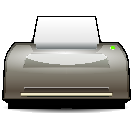
\includegraphics[scale=0.75]{printer.pdf} & Printer server \\ \hline
Paketname & \textbf{cups} \\ 
Repository & official repository(extra) \\
Konfigurationsdatei & - \\
Lizenz & GPL \\
Besonderheiten & Einrichtung und Verwaltung: http://localhost:631 als root \\
\end{tabular}
\\ \\
Für eine gute Auswahl an hochqualitvativen freien Druckertreibern kann Gutenprint \textbf{gutenprint}
aus den official repositories installiert werden:
\begin{lstlisting}[style=Bash]
# pacman -S gutenprint 
\end{lstlisting}
Nun muss noch der Service enabled werden:
\begin{lstlisting}[style=Bash]
# systemctl enable cups
\end{lstlisting}

\subsection{Musicplayer}
\begin{tabular}{l|l|l|l}
~ & Server & Client & Client2 \\ \hline
    Paketname & \textbf{mpd} & \textbf{ncmpcpp} & \textbf{mpc} \\ 
    Konfigurationsdatei & {{\raise.17ex\hbox{$\scriptstyle\mathtt{\sim}$}}.mpd/mpd.conf} & - & - \\
\end{tabular}
\\ \\
MPD Konfiguration:
.mpd nach home kopieren
\begin{lstlisting}[style=Bash]
$ systemctl --user enable mpd
\end{lstlisting}

\subsection{Music engraver}
\begin{tabular}{l|l}
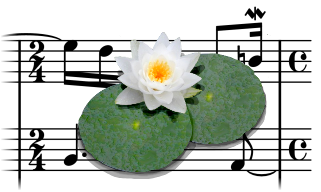
\includegraphics[scale=0.2]{lilypond-logo.png} & Lilypond \\ \hline
Paketname & \textbf{lilypond} \\ 
Repository & official repository(community) \\
Konfigurationsdatei & - \\
Lizenz & GPL \\
Besonderheiten & - \\
\end{tabular}

\subsection{Spiele}
\begin{tabular}{l|l}

\includegraphics[scale=0.25]{steam-logo.pdf} & Steam \\ \hline
Paketname & \textbf{steam} \\ 
Repository & official repository(multilib) \\
Konfigurationsdatei & - \\
Lizenz & custom \\
Besonderheiten & - \\
\end{tabular}
\\ \\ \\
\begin{tabular}{l|l}

\includegraphics[scale=0.25]{minecraft-logo.pdf} & Minecraft \\ \hline
Paketname & \textbf{minecraft} \\ 
Repository & arch user repository \\
Konfigurationsdatei & - \\
Lizenz & custom \\
Besonderheiten & - \\
\end{tabular}



\end{document}
